Since we use a complete set of minimum number of 
input variables necessary to describe the whole event topology, 
these variables are mostly mostly uncorrelated. 
The correlation matrix for signal and background 
samples are shown in Figs~\ref{fig:FigCorr170Mu}--\ref{fig:FigCorr600Mu}
for various Higgs mass points.
%%%%%%%%%%%%%%%%%%%
\subsection{Correlation matrix: \texorpdfstring{$M_H$}{M(H)} = 170~GeV}
%%%%%%%%%%%%%%%%%%%
\begin{figure}[bthp!]
\subfigure[]{
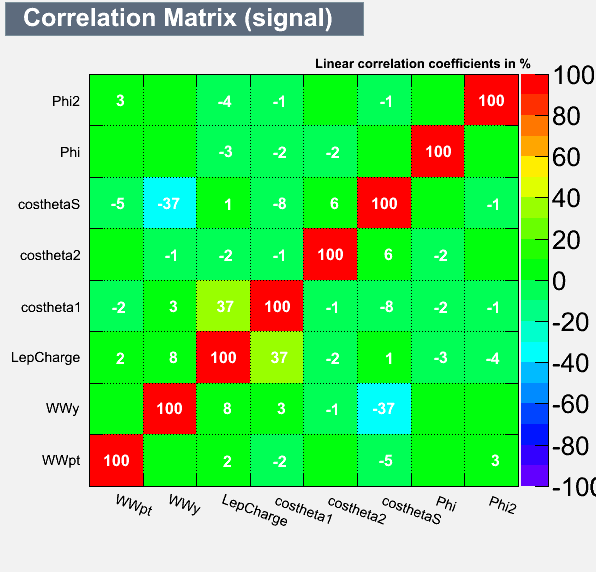
\includegraphics[width=0.49\textwidth]{figs/TMVA_170_nJ2_mu_CorrelationMatrixS}
}
\subfigure[]{
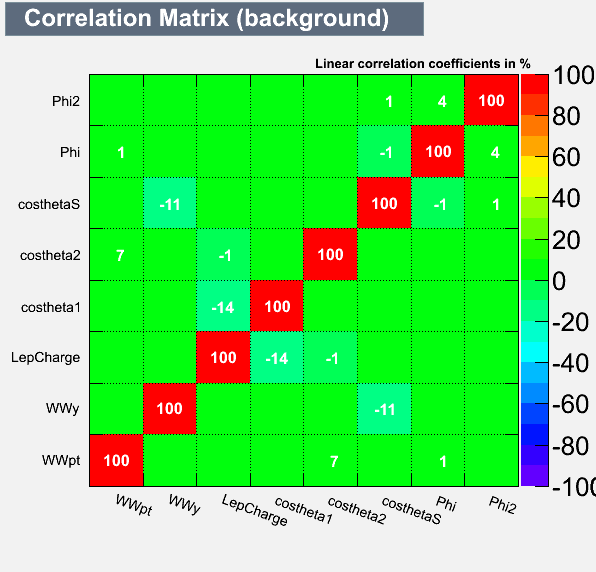
\includegraphics[width=0.49\textwidth]{figs/TMVA_170_nJ2_mu_CorrelationMatrixB}
}
\vspace*{1mm} \\
\subfigure[]{
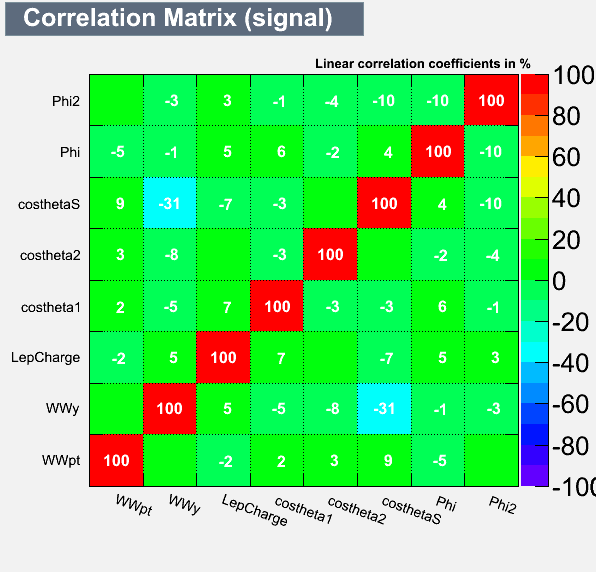
\includegraphics[width=0.49\textwidth]{figs/TMVA_170_nJ3_mu_CorrelationMatrixS}
}
\subfigure[]{
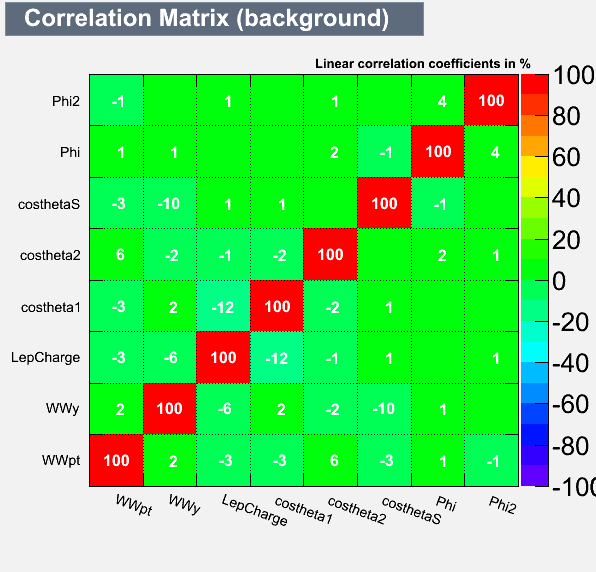
\includegraphics[width=0.49\textwidth]{figs/TMVA_170_nJ3_mu_CorrelationMatrixB}
}
\caption{\label{fig:FigCorr170Mu} 
Correlation matrix for input variables for Higgs mass point 170 GeV:
(a) signal 2 jets, (b) W+jets background 2 jets, 
(c) signal 3 jets, and (d) W+jets background 3 jets.
}
\end{figure}
%%%%%%%%%%%%%%%%%%%
\newpage
\subsection{Correlation matrix: \texorpdfstring{$M_H$}{M(H)} = 180~GeV}
%%%%%%%%%%%%%%%%%%%
\begin{figure}[bthp!]
\subfigure[]{
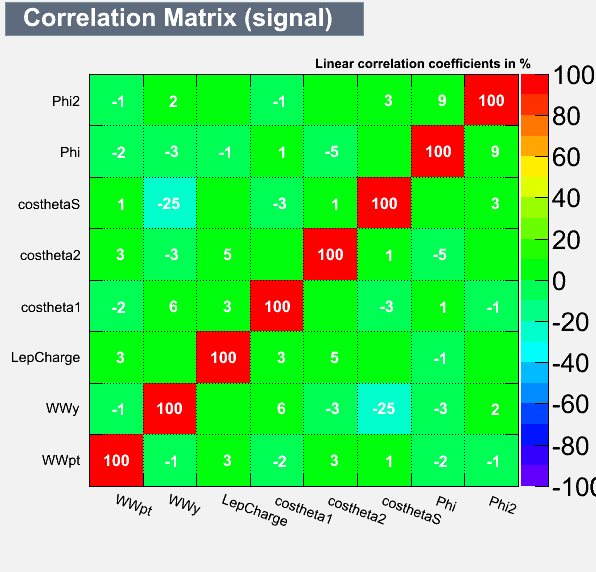
\includegraphics[width=0.49\textwidth]{figs/TMVA_180_nJ2_mu_CorrelationMatrixS}
}
\subfigure[]{
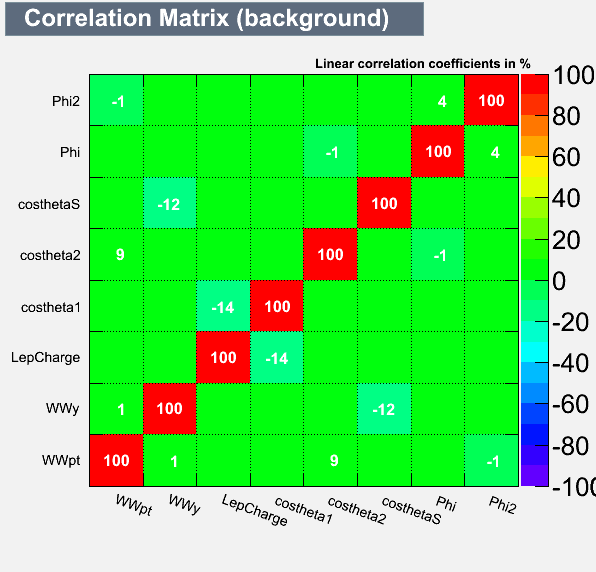
\includegraphics[width=0.49\textwidth]{figs/TMVA_180_nJ2_mu_CorrelationMatrixB}
}
\vspace*{1mm} \\
\subfigure[]{
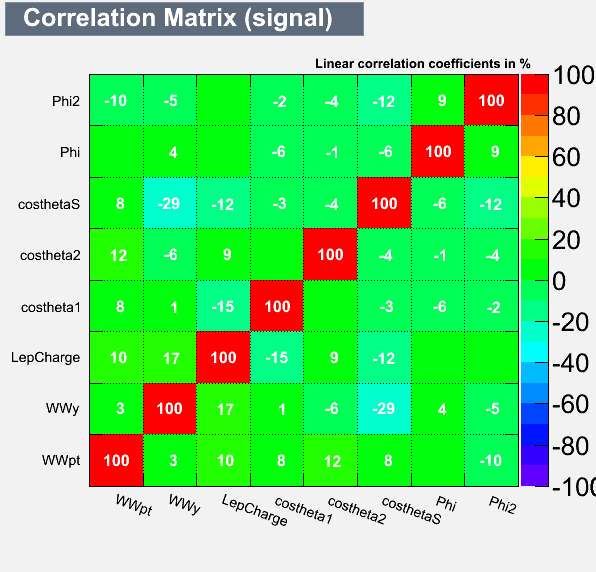
\includegraphics[width=0.49\textwidth]{figs/TMVA_180_nJ3_mu_CorrelationMatrixS}
}
\subfigure[]{
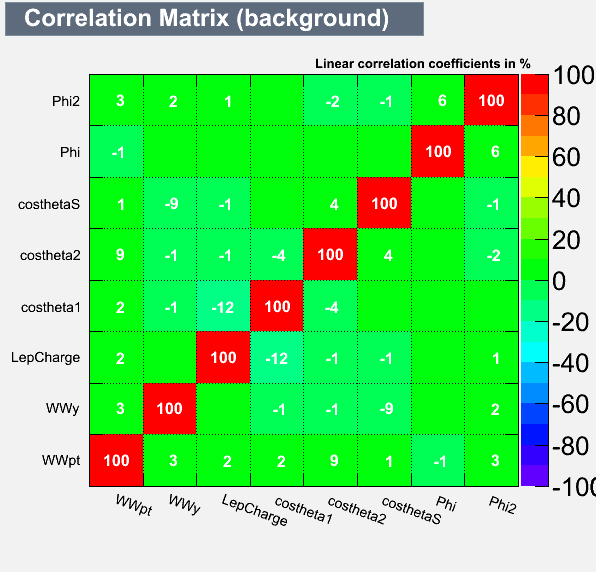
\includegraphics[width=0.49\textwidth]{figs/TMVA_180_nJ3_mu_CorrelationMatrixB}
}
\caption{\label{fig:FigCorr180Mu} 
Correlation matrix for input variables for Higgs mass point 180 GeV:
(a) signal 2 jets, (b) W+jets background 2 jets, 
(c) signal 3 jets, and (d) W+jets background 3 jets.
}
\end{figure}
%%%%%%%%%%%%%%%%%%%
\newpage
\subsection{Correlation matrix: \texorpdfstring{$M_H$}{M(H)} = 190~GeV}
%%%%%%%%%%%%%%%%%%%
\begin{figure}[bthp!]
\subfigure[]{
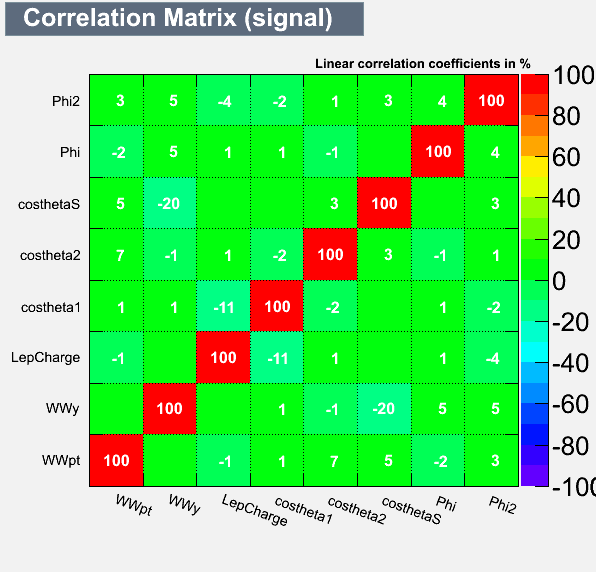
\includegraphics[width=0.49\textwidth]{figs/TMVA_190_nJ2_mu_CorrelationMatrixS}
}
\subfigure[]{
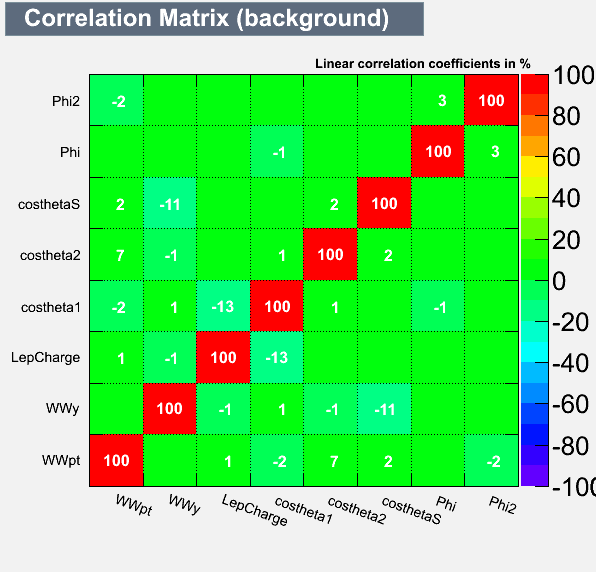
\includegraphics[width=0.49\textwidth]{figs/TMVA_190_nJ2_mu_CorrelationMatrixB}
}
\vspace*{1mm} \\
\subfigure[]{
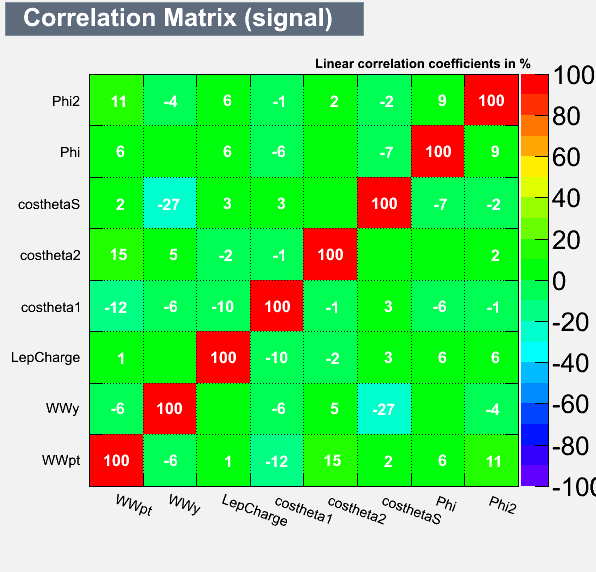
\includegraphics[width=0.49\textwidth]{figs/TMVA_190_nJ3_mu_CorrelationMatrixS}
}
\subfigure[]{
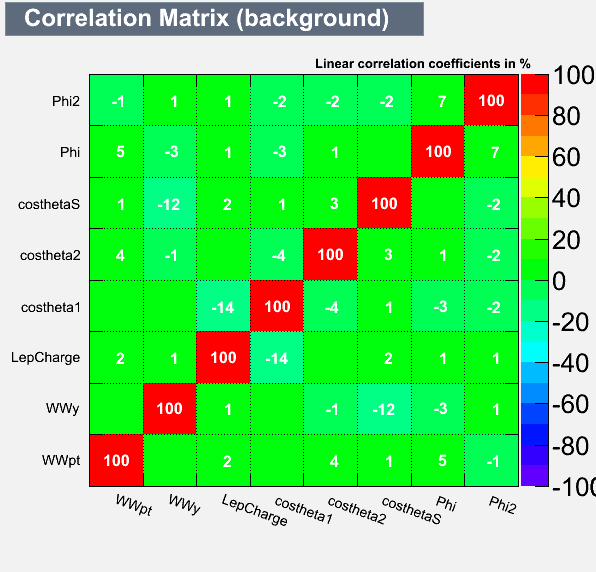
\includegraphics[width=0.49\textwidth]{figs/TMVA_190_nJ3_mu_CorrelationMatrixB}
}


\caption{\label{fig:FigCorr190Mu} 
Correlation matrix for input variables for Higgs mass point 190 GeV:
(a) signal 2 jets, (b) W+jets background 2 jets, 
(c) signal 3 jets, and (d) W+jets background 3 jets.
}
\end{figure}
%%%%%%%%%%%%%%%%%%%
\newpage
\subsection{Correlation matrix: \texorpdfstring{$M_H$}{M(H)} = 200~GeV}
%%%%%%%%%%%%%%%%%%%
\begin{figure}[bthp!]
\subfigure[]{
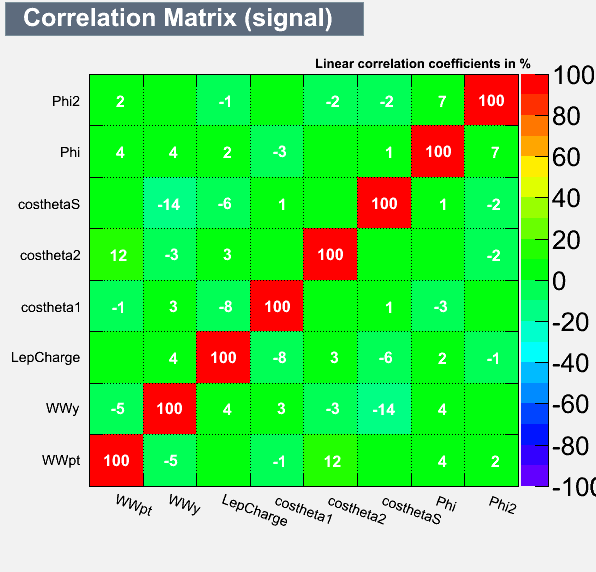
\includegraphics[width=0.49\textwidth]{figs/TMVA_200_nJ2_mu_CorrelationMatrixS}
}
\subfigure[]{
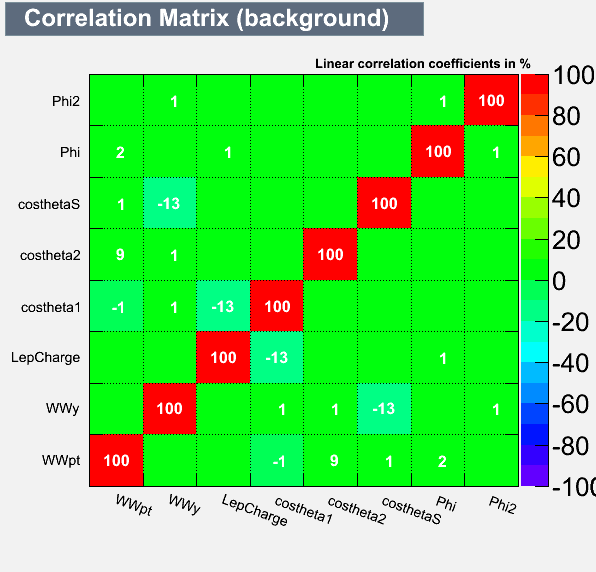
\includegraphics[width=0.49\textwidth]{figs/TMVA_200_nJ2_mu_CorrelationMatrixB}
}
\vspace*{1mm} \\
\subfigure[]{
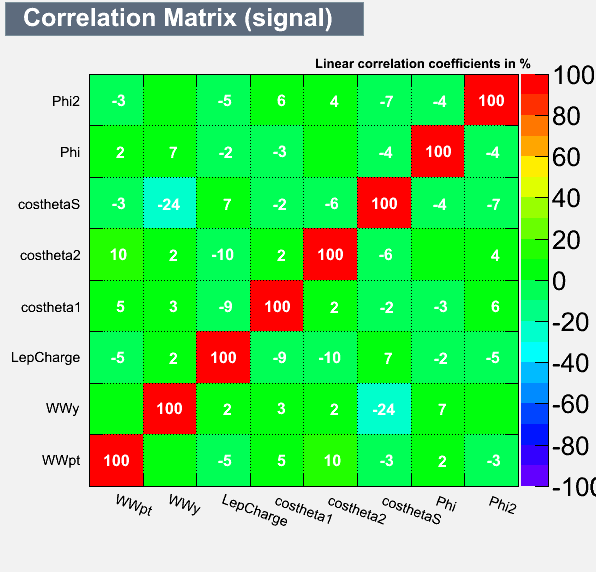
\includegraphics[width=0.49\textwidth]{figs/TMVA_200_nJ3_mu_CorrelationMatrixS}
}
\subfigure[]{
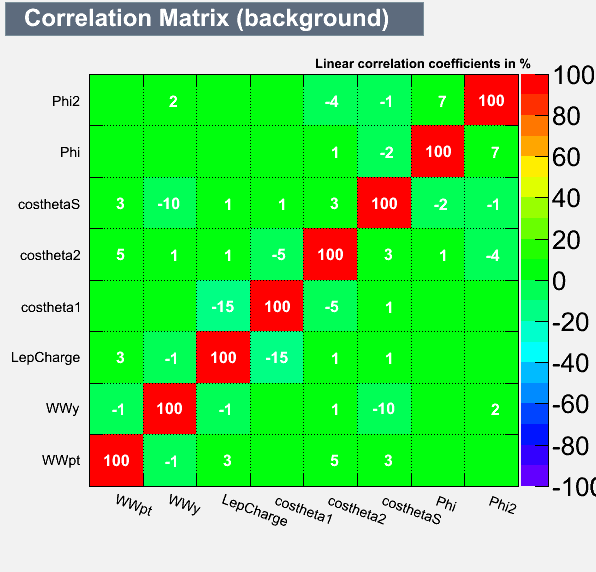
\includegraphics[width=0.49\textwidth]{figs/TMVA_200_nJ3_mu_CorrelationMatrixB}
}


\caption{\label{fig:FigCorr200Mu} 
Correlation matrix for input variables for Higgs mass point 200 GeV:
(a) signal 2 jets, (b) W+jets background 2 jets, 
(c) signal 3 jets, and (d) W+jets background 3 jets.
}
\end{figure}
%%%%%%%%%%%%%%%%%%%
\newpage
\subsection{Correlation matrix: \texorpdfstring{$M_H$}{M(H)} = 250~GeV}
%%%%%%%%%%%%%%%%%%%
\begin{figure}[bthp!]
\subfigure[]{
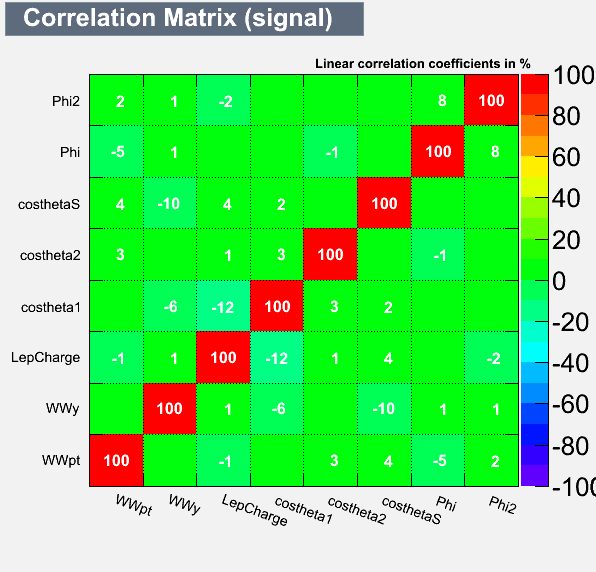
\includegraphics[width=0.49\textwidth]{figs/TMVA_250_nJ2_mu_CorrelationMatrixS}
}
\subfigure[]{
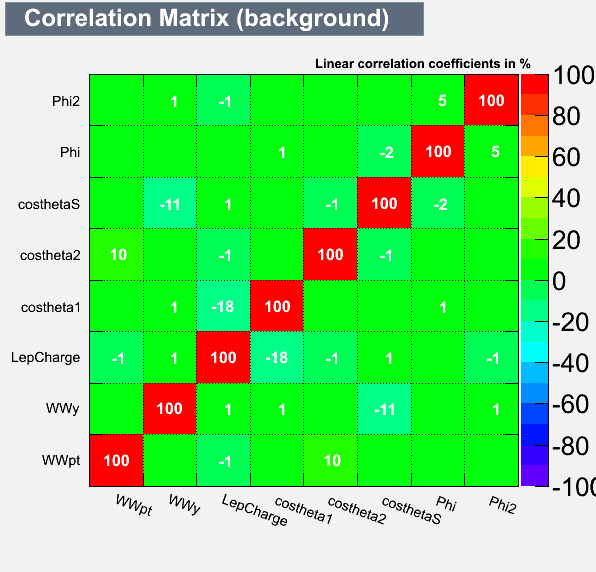
\includegraphics[width=0.49\textwidth]{figs/TMVA_250_nJ2_mu_CorrelationMatrixB}
}
\vspace*{1mm} \\
\subfigure[]{
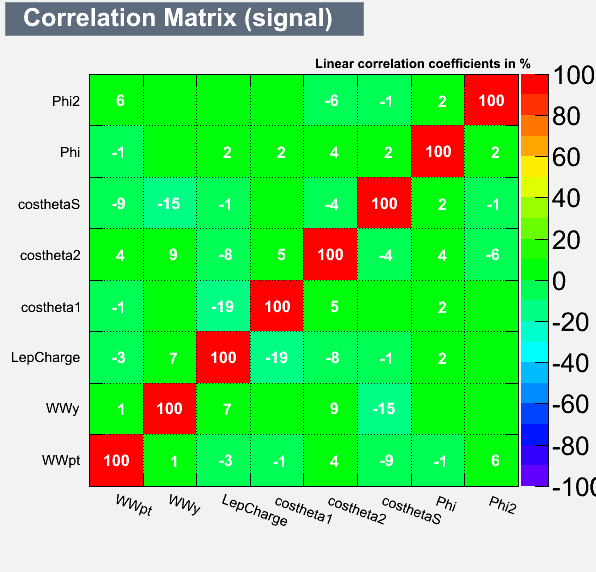
\includegraphics[width=0.49\textwidth]{figs/TMVA_250_nJ3_mu_CorrelationMatrixS}
}
\subfigure[]{
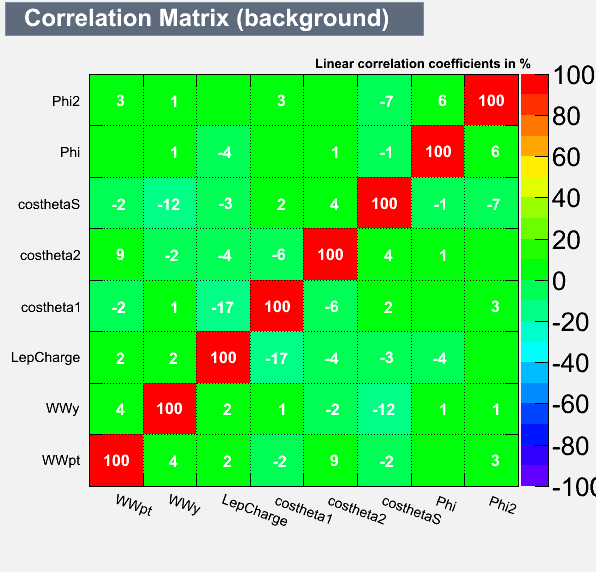
\includegraphics[width=0.49\textwidth]{figs/TMVA_250_nJ3_mu_CorrelationMatrixB}
}


\caption{\label{fig:FigCorr250Mu} 
Correlation matrix for input variables for Higgs mass point 250 GeV:
(a) signal 2 jets, (b) W+jets background 2 jets, 
(c) signal 3 jets, and (d) W+jets background 3 jets.
}
\end{figure}
%%%%%%%%%%%%%%%%%%%
\newpage
\subsection{Correlation matrix: \texorpdfstring{$M_H$}{M(H)} = 300~GeV}
%%%%%%%%%%%%%%%%%%%
\begin{figure}[bthp!]
\subfigure[]{
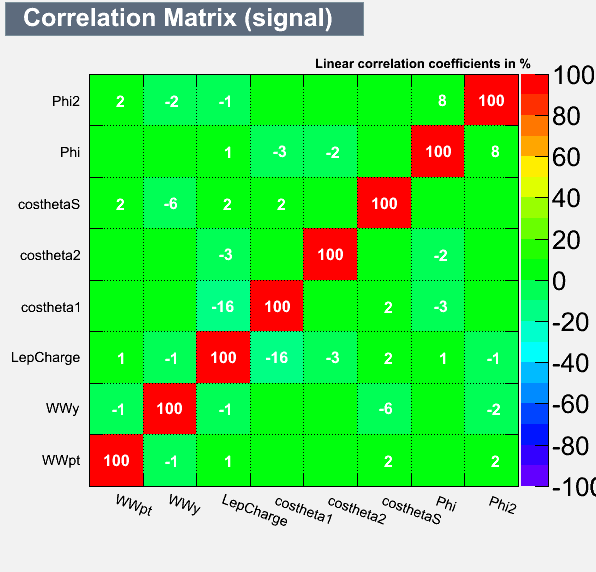
\includegraphics[width=0.49\textwidth]{figs/TMVA_300_nJ2_mu_CorrelationMatrixS}
}
\subfigure[]{
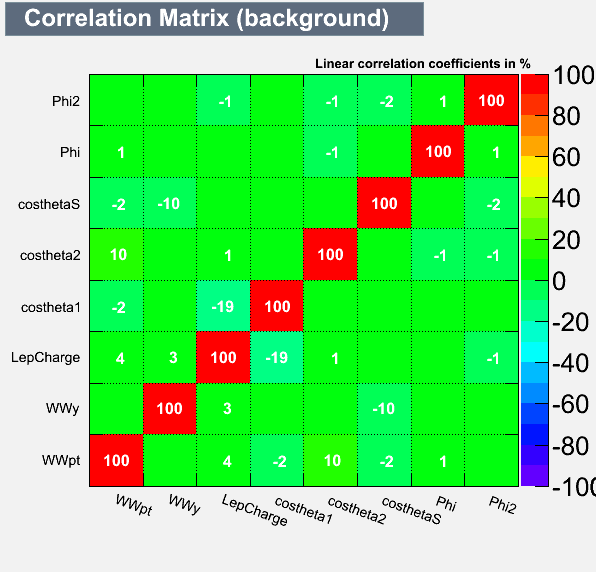
\includegraphics[width=0.49\textwidth]{figs/TMVA_300_nJ2_mu_CorrelationMatrixB}
}
\vspace*{1mm} \\
\subfigure[]{
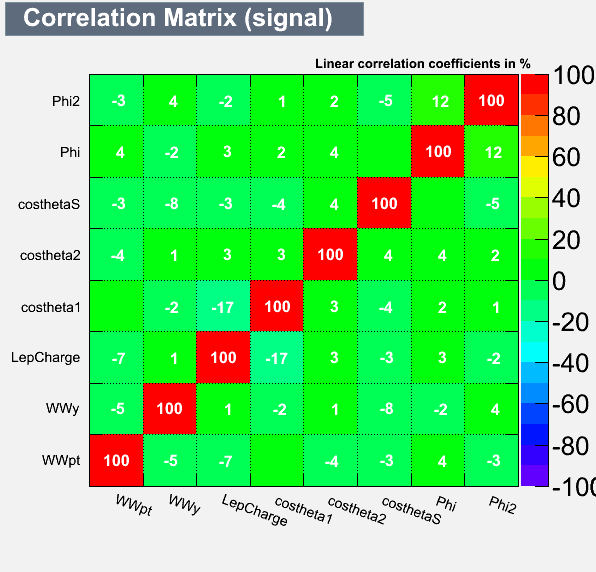
\includegraphics[width=0.49\textwidth]{figs/TMVA_300_nJ3_mu_CorrelationMatrixS}
}
\subfigure[]{
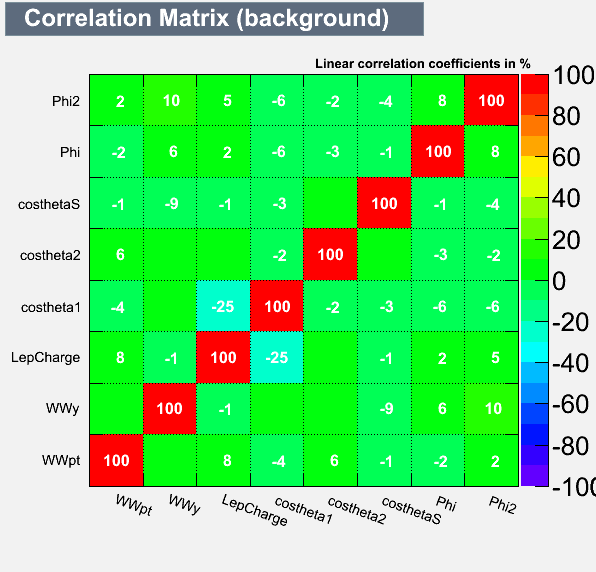
\includegraphics[width=0.49\textwidth]{figs/TMVA_300_nJ3_mu_CorrelationMatrixB}
}


\caption{\label{fig:FigCorr300Mu} 
Correlation matrix for input variables for Higgs mass point 300 GeV:
(a) signal 2 jets, (b) W+jets background 2 jets, 
(c) signal 3 jets, and (d) W+jets background 3 jets.
}
\end{figure}
%%%%%%%%%%%%%%%%%%%
\newpage
\subsection{Correlation matrix: \texorpdfstring{$M_H$}{M(H)} = 350~GeV}
%%%%%%%%%%%%%%%%%%%
\begin{figure}[bthp!]
\subfigure[]{
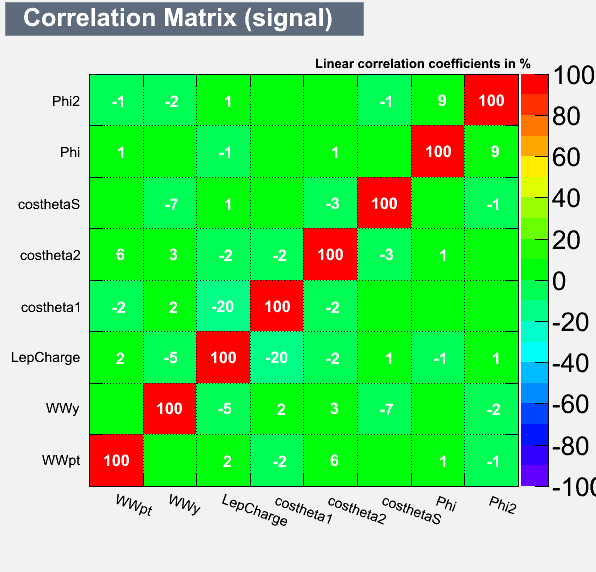
\includegraphics[width=0.49\textwidth]{figs/TMVA_350_nJ2_mu_CorrelationMatrixS}
}
\subfigure[]{
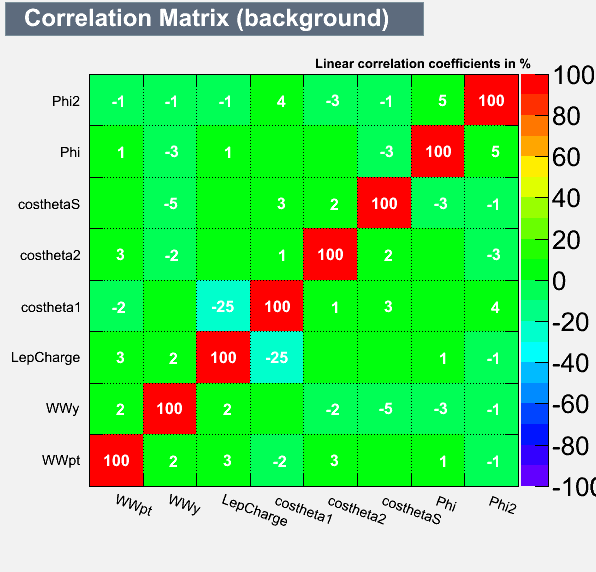
\includegraphics[width=0.49\textwidth]{figs/TMVA_350_nJ2_mu_CorrelationMatrixB}
}
\vspace*{1mm} \\
\subfigure[]{
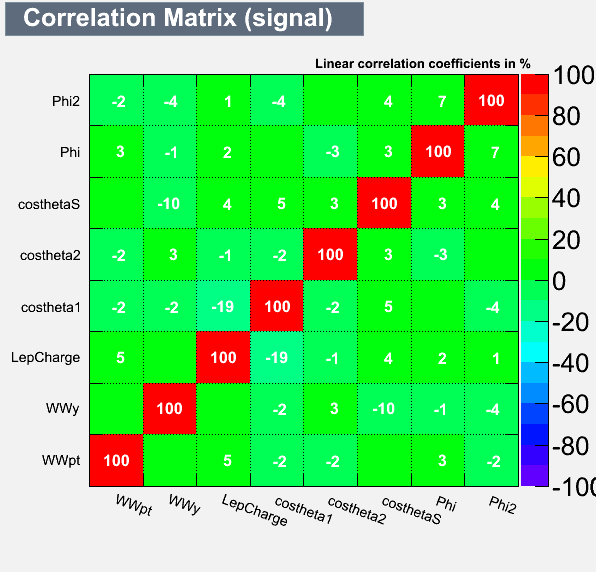
\includegraphics[width=0.49\textwidth]{figs/TMVA_350_nJ3_mu_CorrelationMatrixS}
}
\subfigure[]{
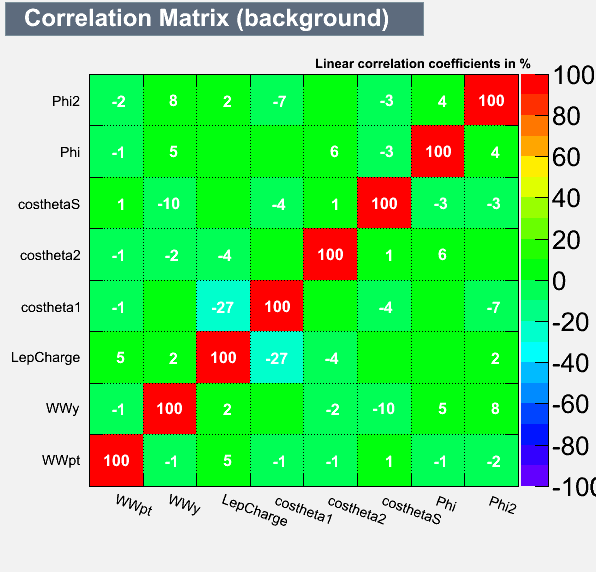
\includegraphics[width=0.49\textwidth]{figs/TMVA_350_nJ3_mu_CorrelationMatrixB}
}


\caption{\label{fig:FigCorr350Mu} 
Correlation matrix for input variables for Higgs mass point 350 GeV:
(a) signal 2 jets, (b) W+jets background 2 jets, 
(c) signal 3 jets, and (d) W+jets background 3 jets.
}
\end{figure}
%%%%%%%%%%%%%%%%%%%
\newpage
\subsection{Correlation matrix: \texorpdfstring{$M_H$}{M(H)} = 400~GeV}
%%%%%%%%%%%%%%%%%%%
\begin{figure}[bthp!]
\subfigure[]{
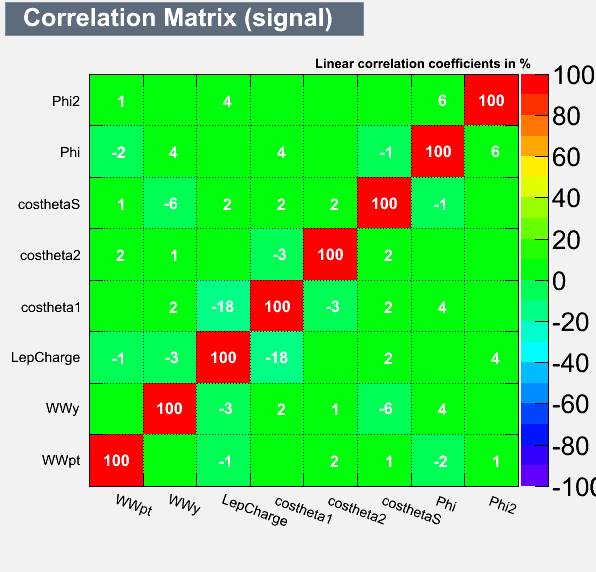
\includegraphics[width=0.49\textwidth]{figs/TMVA_400_nJ2_mu_CorrelationMatrixS}
}
\subfigure[]{
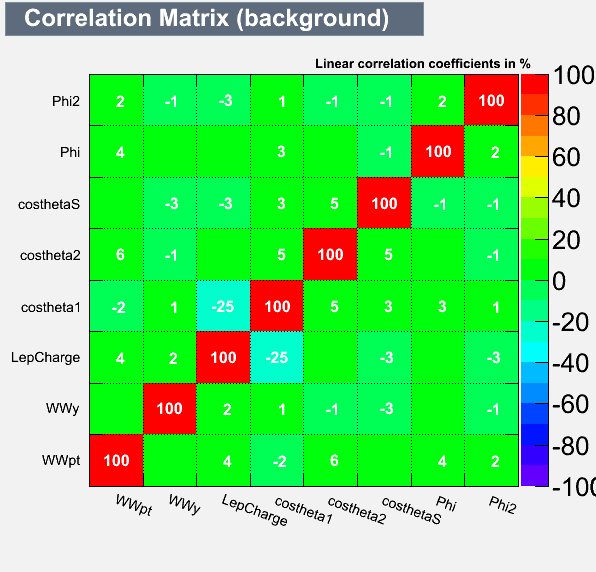
\includegraphics[width=0.49\textwidth]{figs/TMVA_400_nJ2_mu_CorrelationMatrixB}
}
\vspace*{1mm} \\
\subfigure[]{
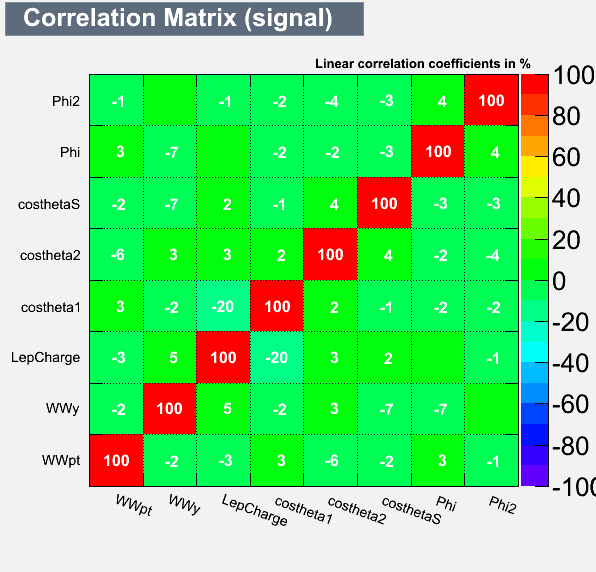
\includegraphics[width=0.49\textwidth]{figs/TMVA_400_nJ3_mu_CorrelationMatrixS}
}
\subfigure[]{
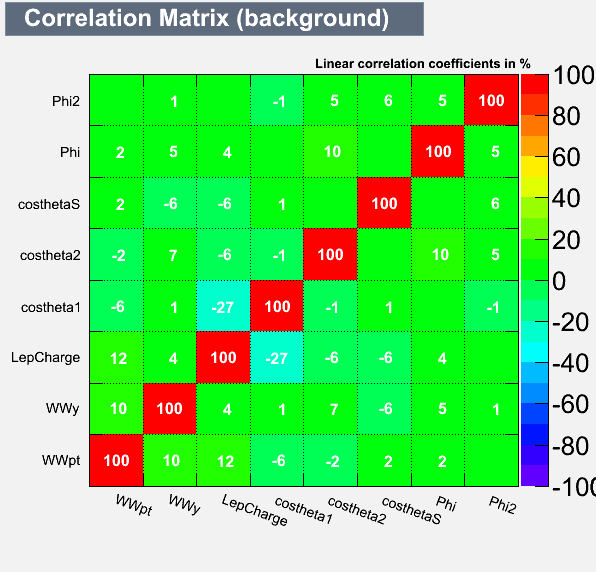
\includegraphics[width=0.49\textwidth]{figs/TMVA_400_nJ3_mu_CorrelationMatrixB}
}


\caption{\label{fig:FigCorr400Mu} 
Correlation matrix for input variables for Higgs mass point 400 GeV:
(a) signal 2 jets, (b) W+jets background 2 jets, 
(c) signal 3 jets, and (d) W+jets background 3 jets.
}
\end{figure}
%%%%%%%%%%%%%%%%%%%
\newpage
\subsection{Correlation matrix: \texorpdfstring{$M_H$}{M(H)} = 450~GeV}
%%%%%%%%%%%%%%%%%%%
\begin{figure}[bthp!]
\subfigure[]{
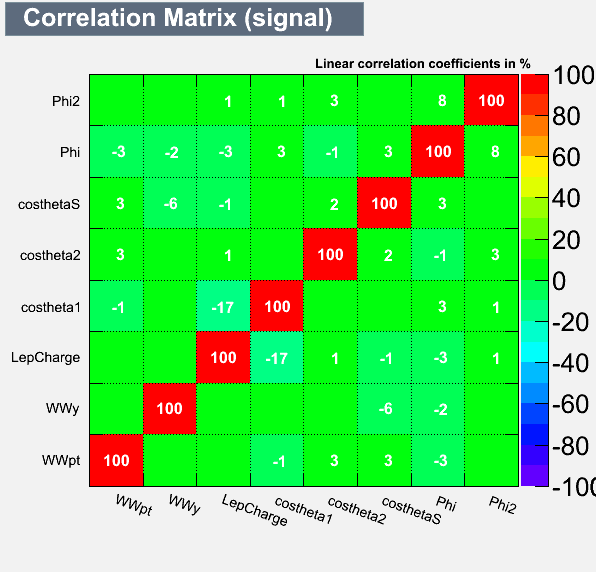
\includegraphics[width=0.49\textwidth]{figs/TMVA_450_nJ2_mu_CorrelationMatrixS}
}
\subfigure[]{
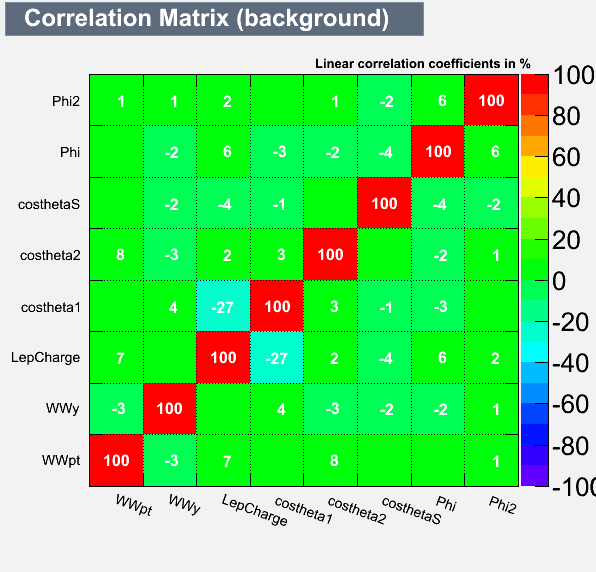
\includegraphics[width=0.49\textwidth]{figs/TMVA_450_nJ2_mu_CorrelationMatrixB}
}
\vspace*{1mm} \\
\subfigure[]{
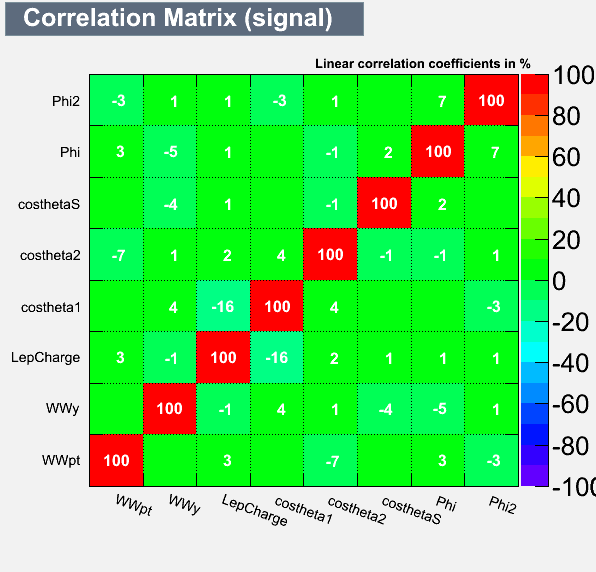
\includegraphics[width=0.49\textwidth]{figs/TMVA_450_nJ3_mu_CorrelationMatrixS}
}
\subfigure[]{
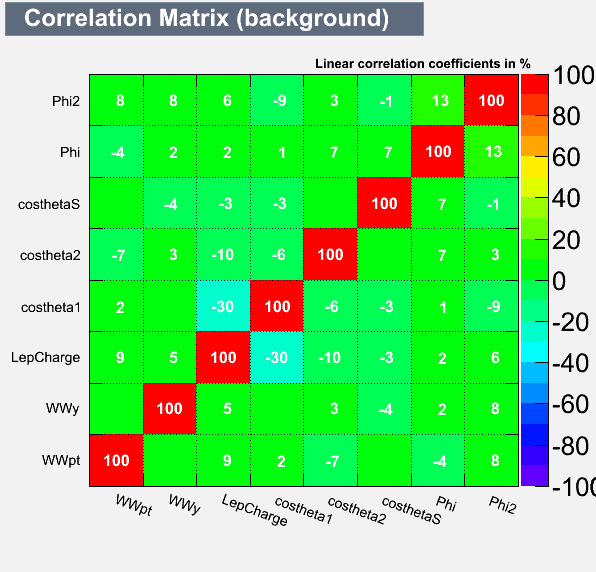
\includegraphics[width=0.49\textwidth]{figs/TMVA_450_nJ3_mu_CorrelationMatrixB}
}


\caption{\label{fig:FigCorr450Mu} 
Correlation matrix for input variables for Higgs mass point 450 GeV:
(a) signal 2 jets, (b) W+jets background 2 jets, 
(c) signal 3 jets, and (d) W+jets background 3 jets.
}
\end{figure}
%%%%%%%%%%%%%%%%%%%
\newpage
\subsection{Correlation matrix: \texorpdfstring{$M_H$}{M(H)} = 500~GeV}
%%%%%%%%%%%%%%%%%%%
\begin{figure}[bthp!]
\subfigure[]{
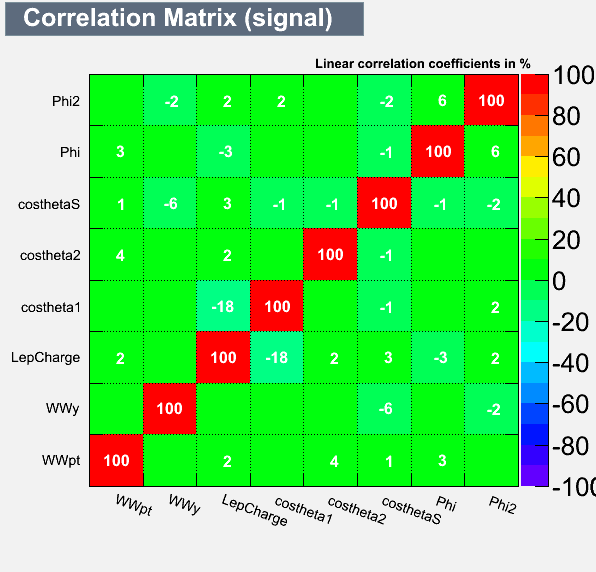
\includegraphics[width=0.49\textwidth]{figs/TMVA_500_nJ2_mu_CorrelationMatrixS}
}
\subfigure[]{
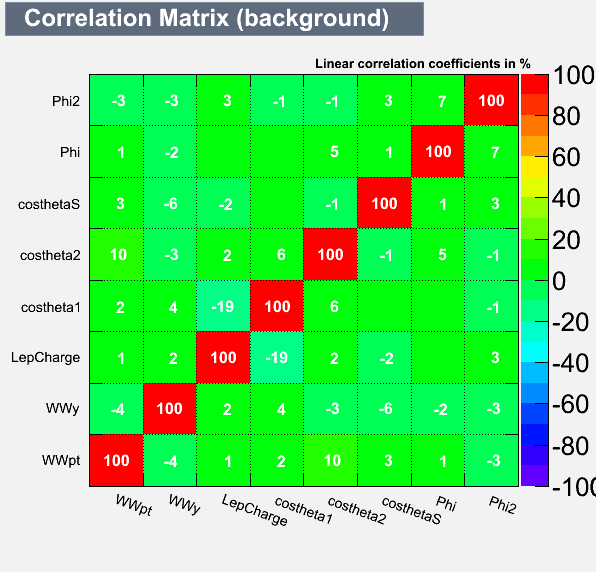
\includegraphics[width=0.49\textwidth]{figs/TMVA_500_nJ2_mu_CorrelationMatrixB}
}
\vspace*{1mm} \\
\subfigure[]{
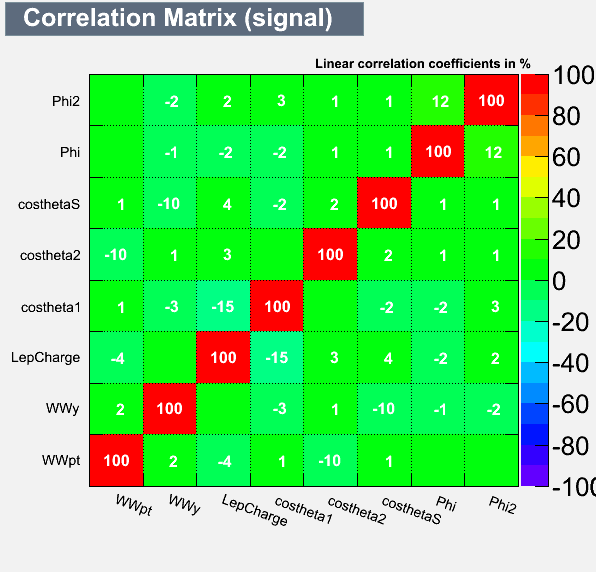
\includegraphics[width=0.49\textwidth]{figs/TMVA_500_nJ3_mu_CorrelationMatrixS}
}
\subfigure[]{
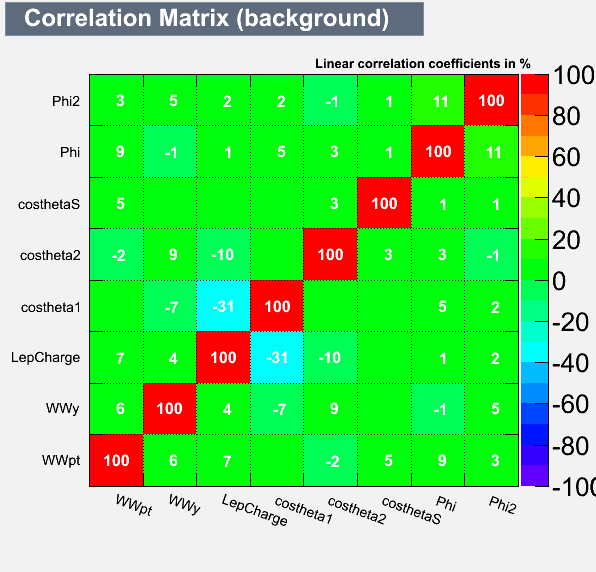
\includegraphics[width=0.49\textwidth]{figs/TMVA_500_nJ3_mu_CorrelationMatrixB}
}


\caption{\label{fig:FigCorr500Mu} 
Correlation matrix for input variables for Higgs mass point 500 GeV:
(a) signal 2 jets, (b) W+jets background 2 jets, 
(c) signal 3 jets, and (d) W+jets background 3 jets.
}
\end{figure}
%%%%%%%%%%%%%%%%%%%
\newpage
\subsection{Correlation matrix: \texorpdfstring{$M_H$}{M(H)} = 550~GeV}
%%%%%%%%%%%%%%%%%%%
\begin{figure}[bthp!]
\subfigure[]{
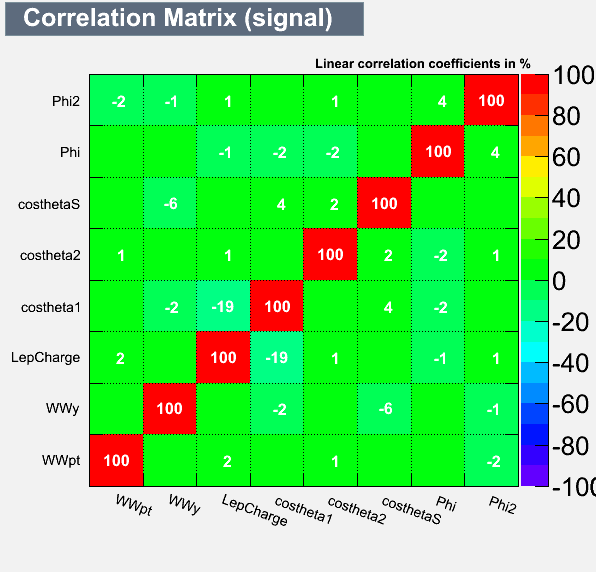
\includegraphics[width=0.49\textwidth]{figs/TMVA_550_nJ2_mu_CorrelationMatrixS}
}
\subfigure[]{
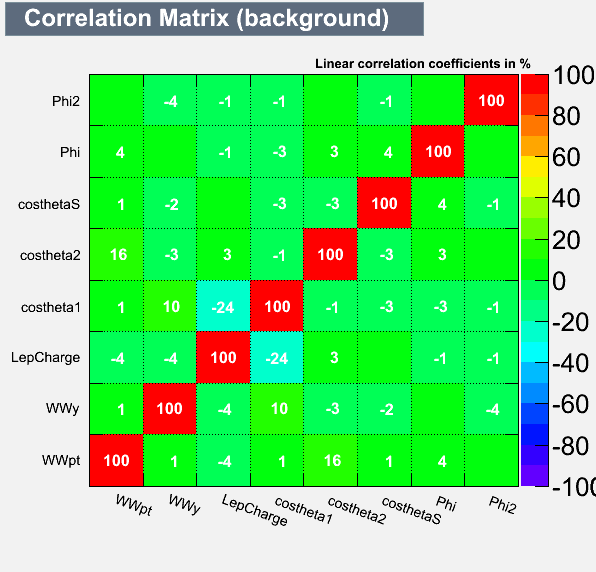
\includegraphics[width=0.49\textwidth]{figs/TMVA_550_nJ2_mu_CorrelationMatrixB}
}
\vspace*{1mm} \\
\subfigure[]{
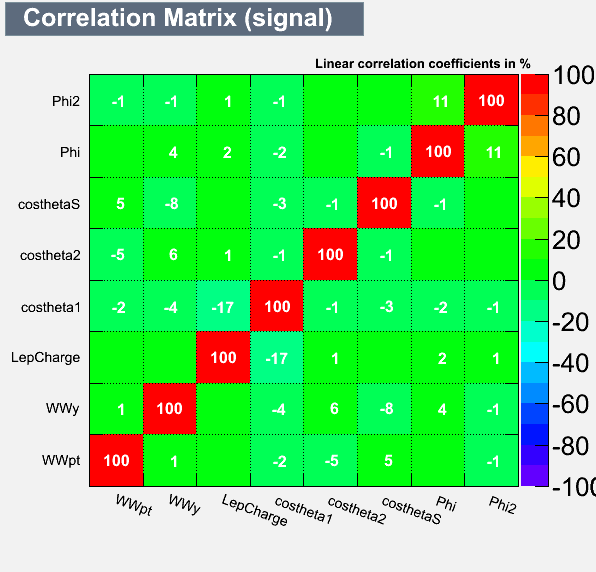
\includegraphics[width=0.49\textwidth]{figs/TMVA_550_nJ3_mu_CorrelationMatrixS}
}
\subfigure[]{
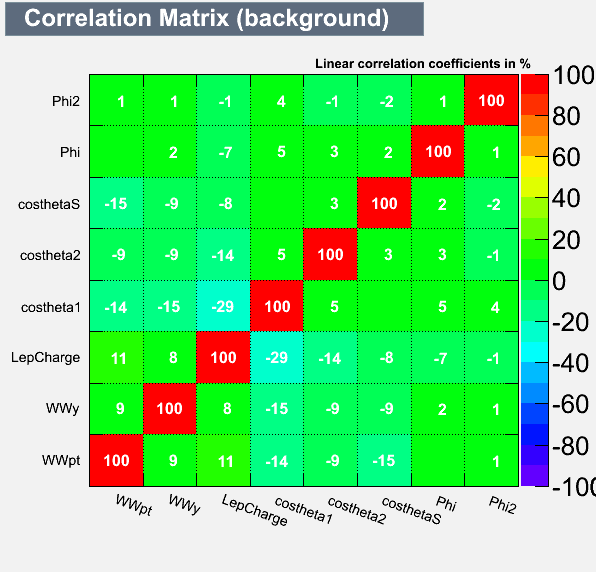
\includegraphics[width=0.49\textwidth]{figs/TMVA_550_nJ3_mu_CorrelationMatrixB}
}


\caption{\label{fig:FigCorr550Mu} 
Correlation matrix for input variables for Higgs mass point 550 GeV:
(a) signal 2 jets, (b) W+jets background 2 jets, 
(c) signal 3 jets, and (d) W+jets background 3 jets.
}
\end{figure}
%%%%%%%%%%%%%%%%%%%
\newpage
\subsection{Correlation matrix: \texorpdfstring{$M_H$}{M(H)} = 600~GeV}
%%%%%%%%%%%%%%%%%%%
\begin{figure}[bthp!]
\subfigure[]{
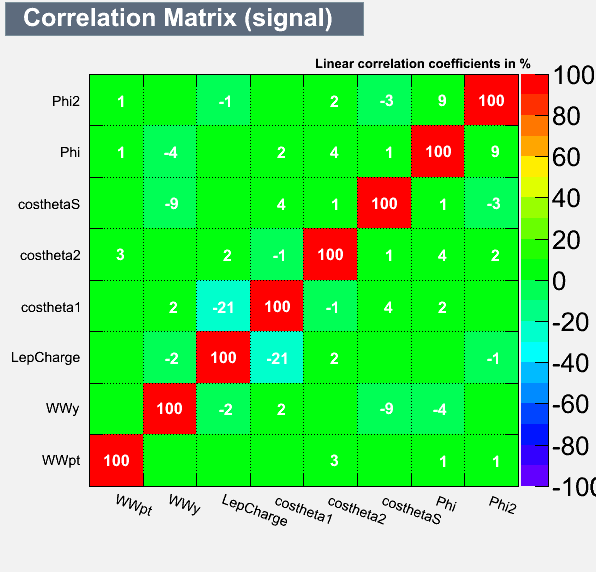
\includegraphics[width=0.49\textwidth]{figs/TMVA_600_nJ2_mu_CorrelationMatrixS}
}
\subfigure[]{
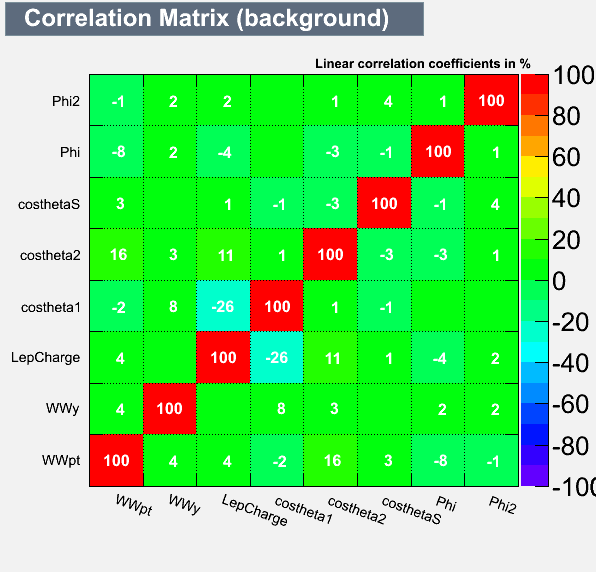
\includegraphics[width=0.49\textwidth]{figs/TMVA_600_nJ2_mu_CorrelationMatrixB}
}
\vspace*{1mm} \\
\subfigure[]{
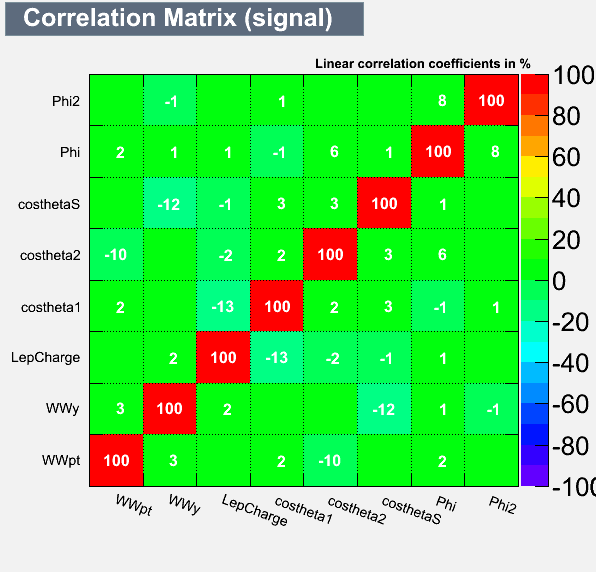
\includegraphics[width=0.49\textwidth]{figs/TMVA_600_nJ3_mu_CorrelationMatrixS}
}
\subfigure[]{
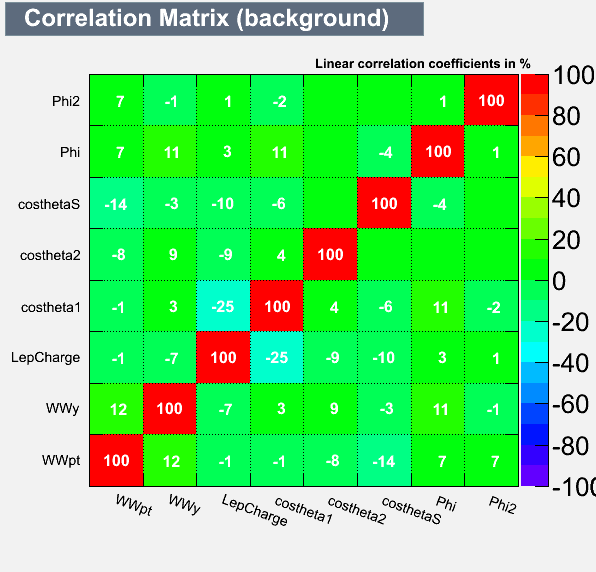
\includegraphics[width=0.49\textwidth]{figs/TMVA_600_nJ3_mu_CorrelationMatrixB}
}


\caption{\label{fig:FigCorr600Mu} 
Correlation matrix for input variables for Higgs mass point 600 GeV:
(a) signal 2 jets, (b) W+jets background 2 jets, 
(c) signal 3 jets, and (d) W+jets background 3 jets.
}
\end{figure}
%%%%%%%%%%%%%%%%%%%
